\documentclass[11pt]{article}
\usepackage[utf8]{inputenc}
\usepackage[margin=0.8in]{geometry}
\usepackage{amsfonts, amsmath}
\usepackage{tikz}
\usepackage[nobreak=false]{mdframed}
\usepackage{pgf}
\usepackage{mathtools}
\usepackage{bbm}
\usepackage{graphicx}
\usepackage{url}
\usepackage{enumerate}
\usepackage{amsthm,amssymb}
\usepackage{minted}
\setlength\parindent{0pt}
\newcommand{\solution}{\subsection*{Solution:}}
\newcommand{\Lagr}{\mathcal{L}}

\begin{document}

\title{EE 240C Homework 2}
\author{Vighnesh Iyer}
\date{\today}
\maketitle

\subsection*{Problem 1: Spectral Analysis}
\begin{enumerate}[a)]
    \item Plot the spectrum from 0 to $f_s/2$ using FFT without averaging. The y-axis should be in dBFS while the x axis should be in MHz.

      \begin{center}
        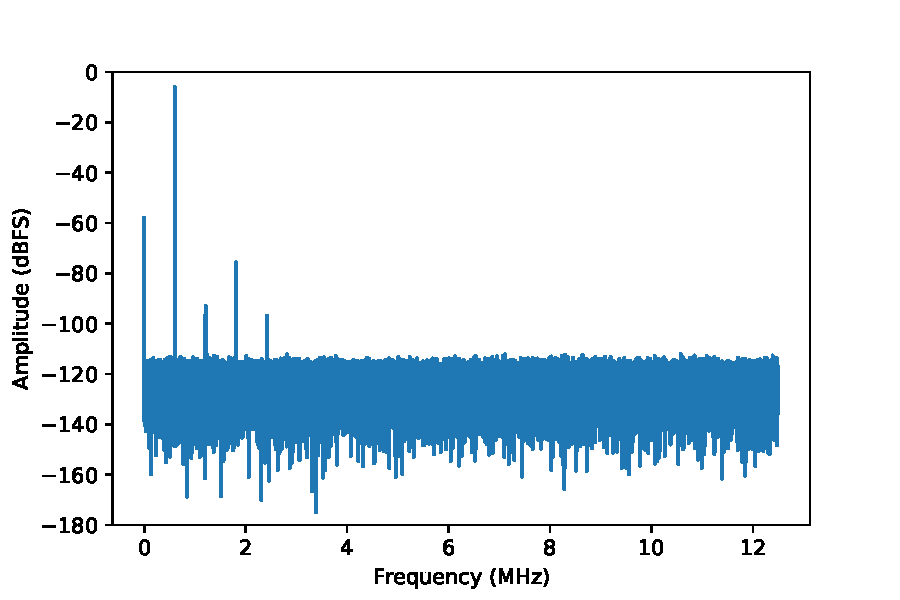
\includegraphics[width=0.6\textwidth]{figs/problem1a.pdf}
      \end{center}

    \item What is the frequency $f_{in}$ of the sinusoidal signal at the input of the ADC?

      The frequency bin with the maximum amplitude is 3171 which corresponds to a frequency of 0.605 MHz.

    \item Compute the following metrics: SNR, SNDR, ENOB, THD, SFDR.

      \begin{itemize}
        \item SNR = $\frac{P_{sig}}{P_{noise}}$ where $P_{noise}$ excludes DC, the signal, and the 2-7th harmonic.

        SNR = $67.9 \text{ dB}$.

        \item SNDR = $\frac{P_{sig}}{P_{noise}}$ where $P_{noise}$ excludes DC and the signal, but includes the harmonics.

          SNDR = $65.65 \text{ dB}$. This is close to the SNR which makes sense since the harmonics are well below the signal.

        \item ENOB = $\frac{SNDR(dB) - 1.76 dB}{6.02 dB}$ = 10.6 bits

        \item THD = $\frac{P_{distortion}}{P_{sig}}$ = -69.5 dB

        \item SFDR = $\frac{P_{spur,max}}{P_{sig}}$ = 69.6 dB
      \end{itemize}

    \item Which non-ideality is limiting the SFDR in this case?

      The INL seems to limiting the SFDR. From the equation in lecture $SFDR = 20 \log_{10}(2^B / INL)$ which for a 12-bit ADC and 1 LSB of INL equals 72 dB SFDR, which is close to the computed value.
\end{enumerate}

\subsection*{Problem 2: Current Steering DACs}

\end{document}
